\section{Versuch 4 - Aufmerksamkeitsmessung}
\label{VideoAnalyse}
Für den Versuch wurde ein Video verwendet, welches ein bewegtes Kreuz zeigt, das als Ziel der Aufmerksamkeit dient. Dieses Kreuz sollten die Probanden normal im Auge behalten, damit für jeden Zeitpunkt bekannt ist wo das Ziel der Aufmerksamkeit liegt.\\
Die Anordnung der Eckpunkte des bewegten Zieles sind in \autoref{img_targets} dargestellt und wurden mittels eines Projektors auf eine Größe von $2,88 \times 1,49 m$ gebracht.\\
Das Ziel welches betrachtet werden soll (Target) beginnt immer in der Mitte und bleibt dort $1s$ stehen, bewegt sich innerhalb von 4 Sekunden zu einen der Randpunkte, verweilt dort für eine Sekunde und begibt sich in $4s$ zu einem nächstgelegenen Randpunkt, bleibt dort $1s$ und geht zurück zum Zentrum, dies wiederholt sich für alle Eckpunkte. Ein gesamter Durchlauf dauert $2min$ und $1s$.\\
Die Versuchspersonen befinden sich etwa $1,5m$ vor der Leinwand, die Kamera befand sich $24cm$ unterhalb und $12,5cm$ vor dem zentralen Punkt des Targets mit Blickrichtung zum Projektor und Personen, siehe \autoref{img_Versuchsaufbau}.\\
Als Aufnahmegerät wurde die Logitech c920 HD Pro Webcam verwendet, diese liefert ein $15FPS$ Video mit einer Auflösung von $1600\times 896$ Pixel und besitzt einen horizontalen Blickwinkel von etwa $70^\circ$.\\
\begin{figure}
	\centering
	\fbox{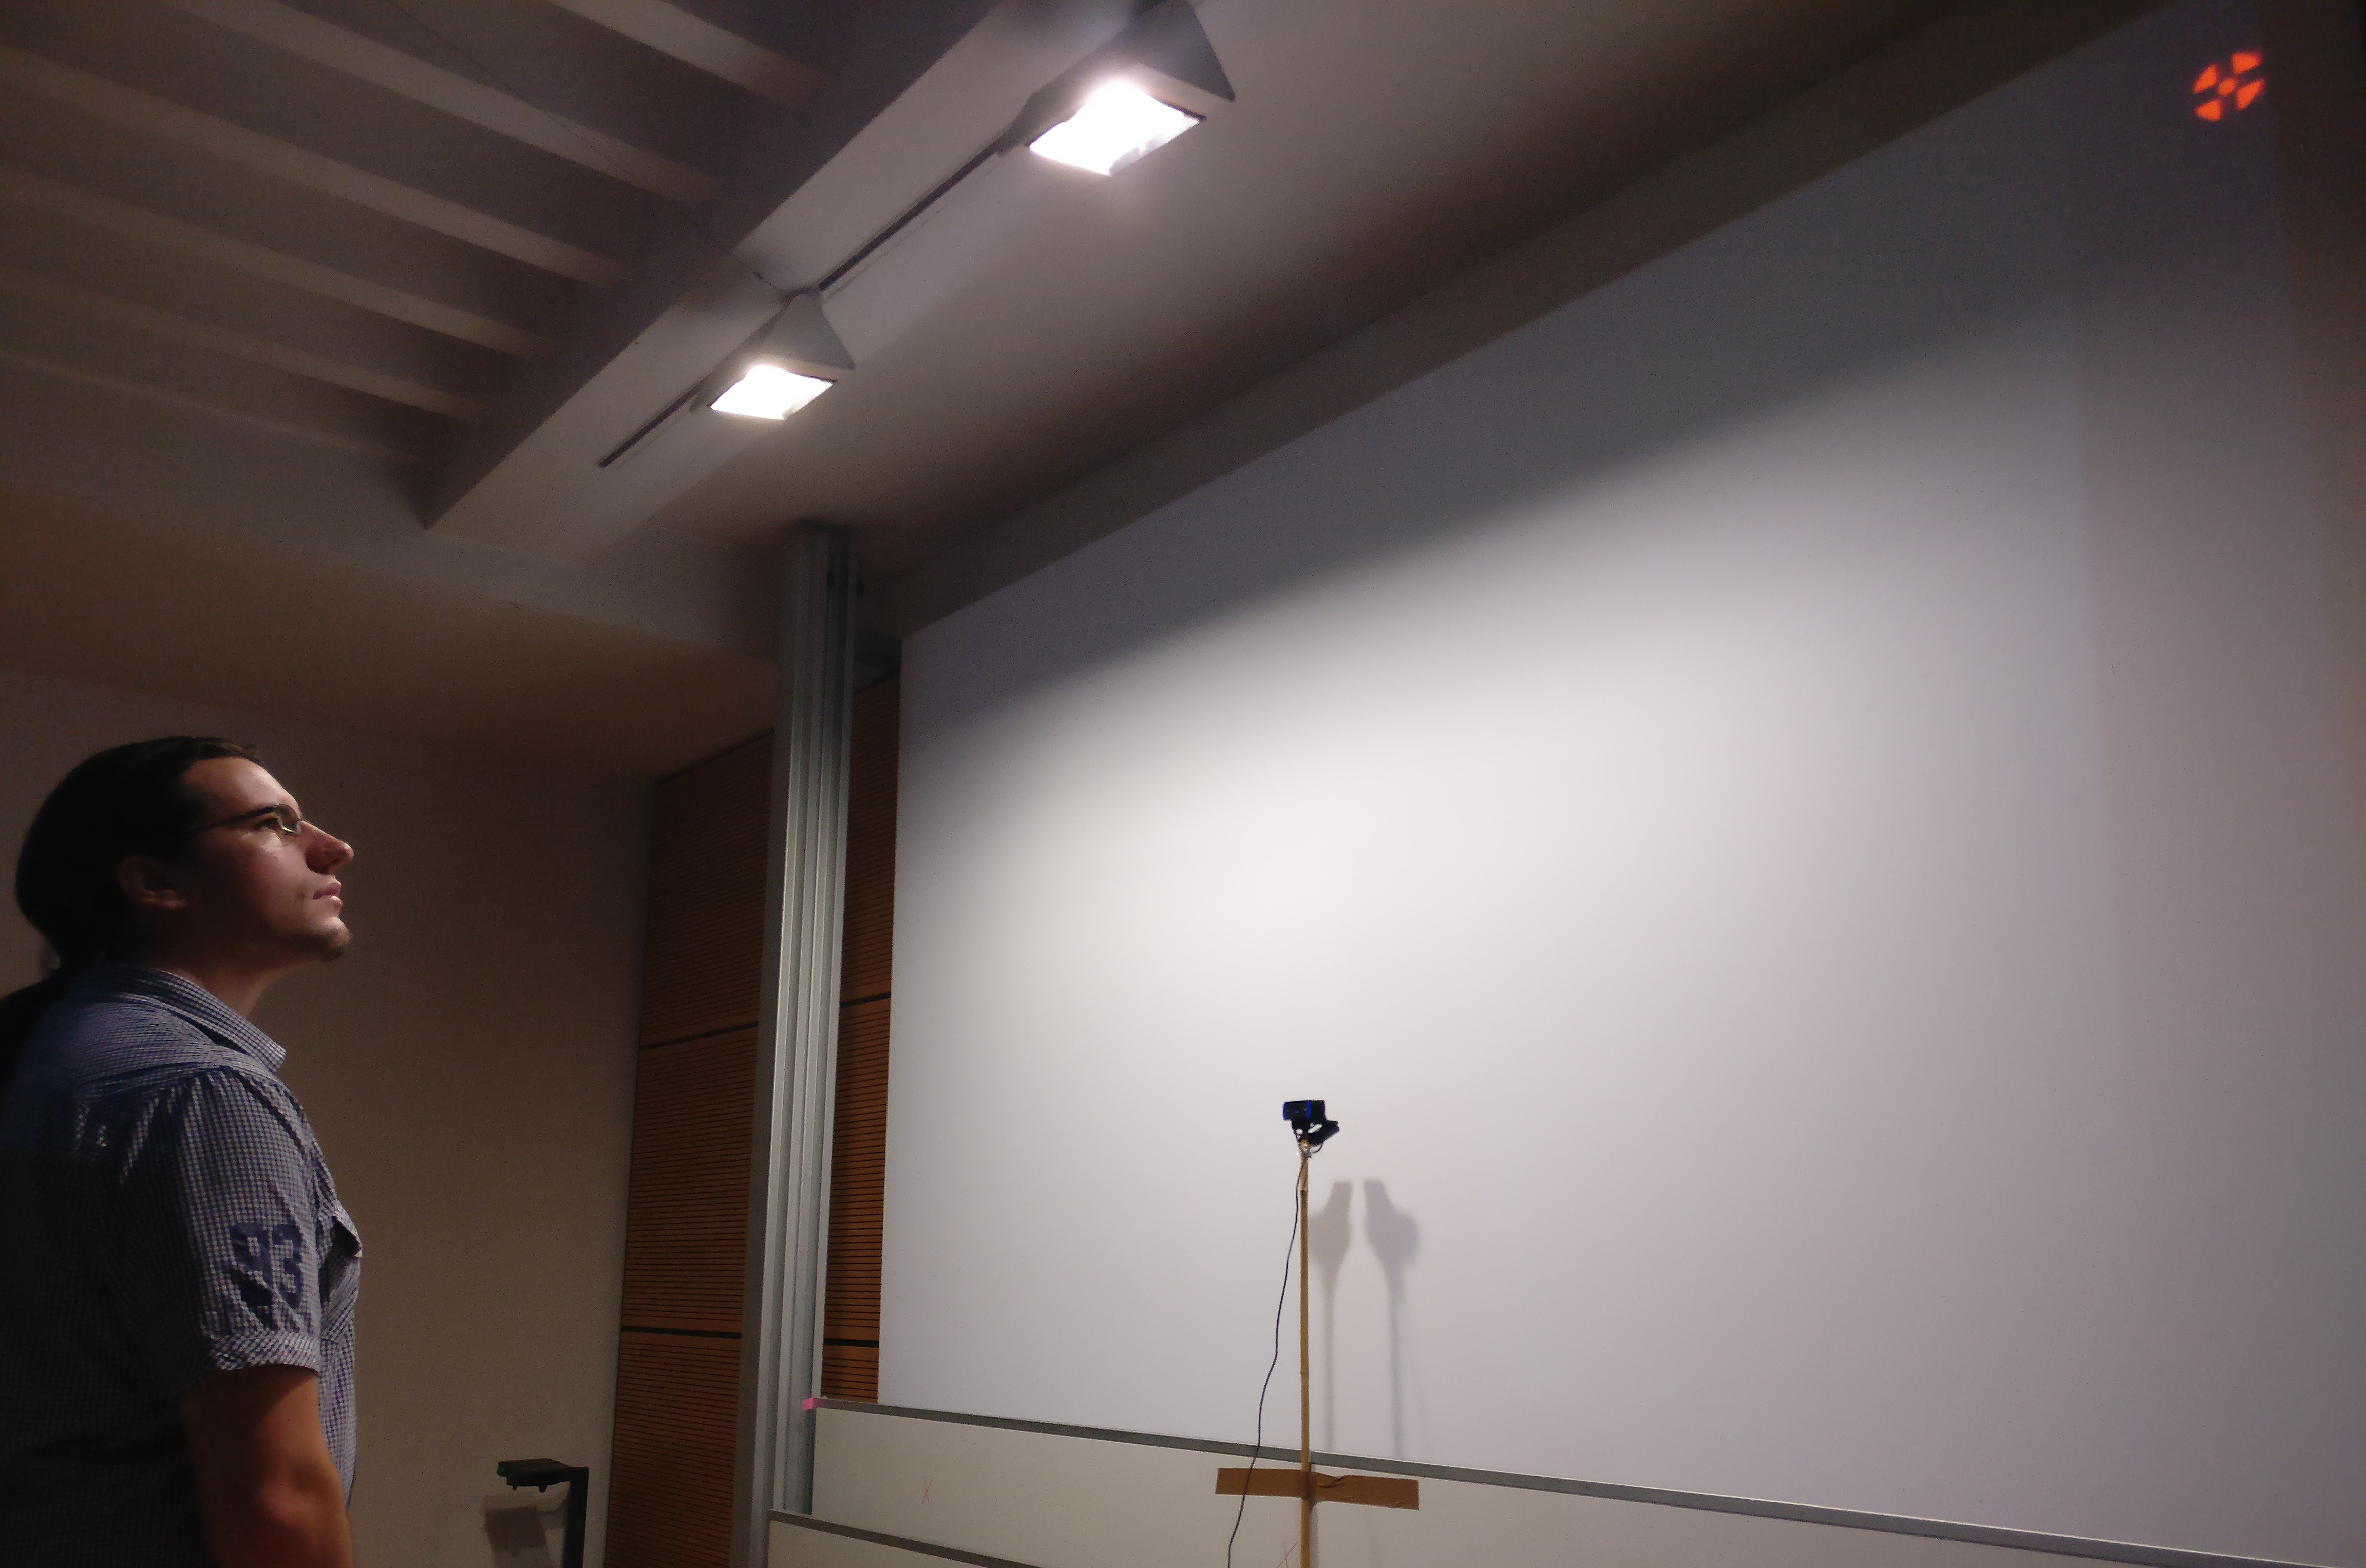
\includegraphics[width=0.7\linewidth]{img/Versuchsaufbau}}
	\caption{Foto der Versuchsdurchführung}
	\label{img_Versuchsaufbau}
\end{figure}
\begin{figure}
\centering
\fbox{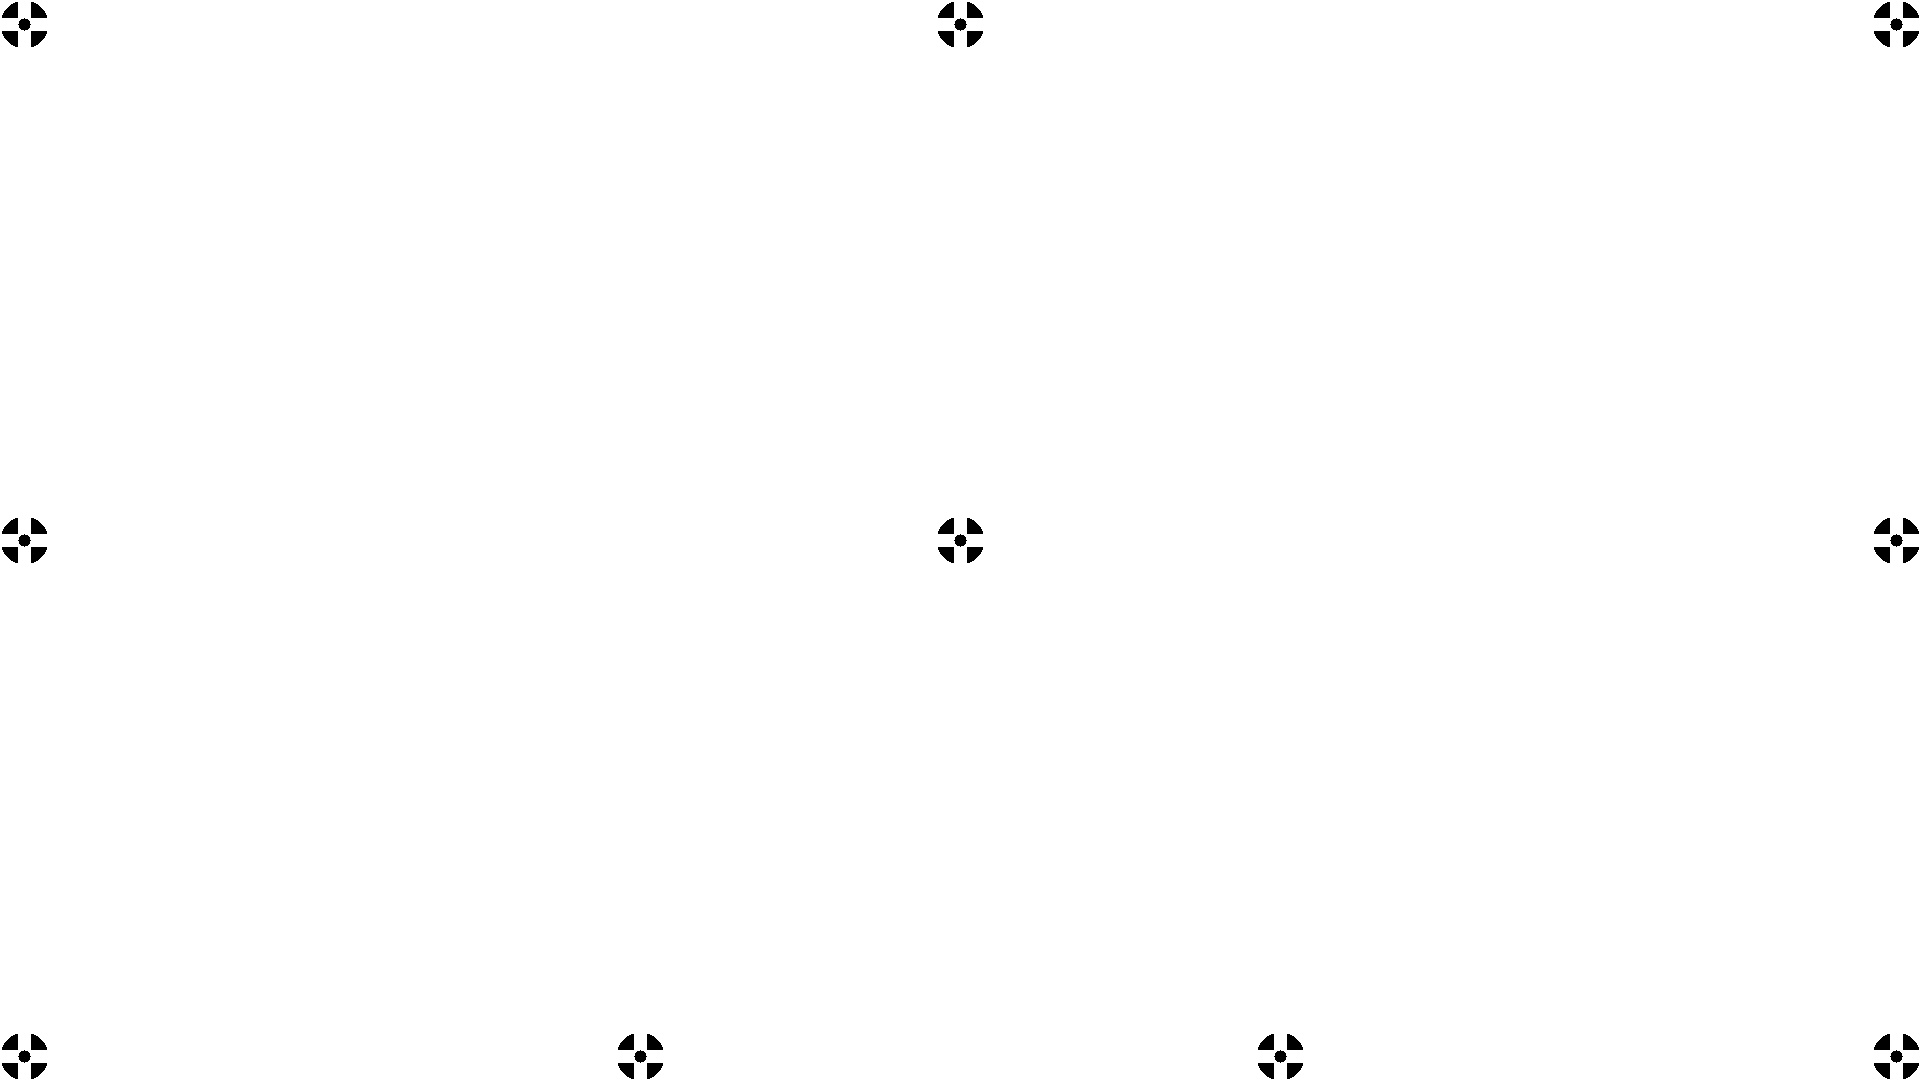
\includegraphics[width=0.7\linewidth]{img/Targets}}
\caption{Eckpositionen des bewegten Zieles bei der Videoaufnahme}
\label{img_targets}
\end{figure}
\subsection{Versuchsdurchführung}
Um die ungefähre Position des Kopfes relativ zur Leinwand zu bestimmen, wurde die Distanz zwischen der Stirn am Nasenrücken und den 4 Eckpunkten durch einen Laserdistanzmessers bestimmt und trianguliert. Während der Aufnahme wurde auf eine weitere Messung der exakten Position verzichtet.\\
Es wurden 8 Videos von 6 Probanden (5 Männlich, 1 Weiblich, 3 mit Brille und 5 ohne Brille) erstellt.\\
Um die Bewegung des Targets mit der Aufzeichnung der Kopfbewegung zu synchronisieren, war im Kamerabild der duplizierte Bildschirm zum Projektorbild zusehen.
\subsubsection{Erster Eindruck}
Dargestellt in \autoref{img_videosumme} sind alle Auftreffpunkte der Blickrichtung auf die Leinwand währen der gesamten Aufnahme.\\
Es ist zu erkennen, dass die eigentlichen Kopfbewegungen sichtbar sind, es aber vor allem in den Randbereichen zu einer großen Differenz kommt.\\
\begin{figure}
	\centering
	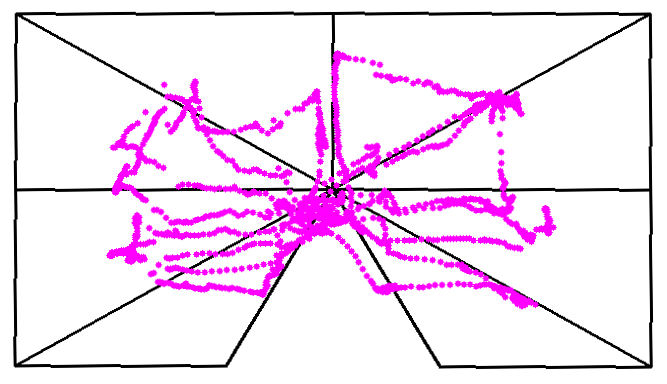
\includegraphics[width=0.7\linewidth]{OpenFace_Img/VideoSumme}
	\caption{Dargestellt sind alle gemessene Auftreffpunkte der Gesichtsorientierung auf die Leinwand (rosa) und des Targets (schwarz)}
	\label{img_videosumme}
\end{figure}
\subsubsection{Qualität}
Durch die begrenzte Auflösung der Kamera und den großen Distanzbereich auf dem gearbeitet werden muss, ist vor allem die Stabilität bezüglich Skalierung wichtig.\\
Bei der Bestimmung des horizontalen Winkels der Kopforientierung zeigt sich, dass die berechneten Werte im Schnitt etwas zu gering ausfallen. Die Orientierung in Richtung Kamera kann zuverlässig bestimmt werden, ebenso wenn der Proband seinen Kopf in eine Richtung dreht. Dabei wird der Fehler um so stärker je größer der zu messende Winkel wird. Betrachtet man in der Originalgröße die jeweiligen Quartale (\autoref{graph_VideoSkalierung}), so sind diese etwa $5^\circ$ auseinander. Genug um einzelne Bereiche differenzieren zu können.\\
Bei der Bestimmung des vertikalen Winkels zeigt sich, dass dieser Wert nur sehr ungenau bestimmt werden konnte, vor allem der Winkel nach oben ist fast nicht messbar. Jener Richtung Boden wird besser erfasst, allerdings ist, bedingt durch den Versuchsausbau, der Wertebereich recht gering.\\
Die bestimmte Blickrichtung ist, trotz Verbesserung durch ElSe und Mittlung beider Augen, schon in der Originalgröße nur begrenzt verwendbar. Die Mittelwerte liegen selbst bei den maximal Werten sehr eng beieinander und die Bereiche überschneiden sich stark. Die Differenz der Mittelwerte zwischen den Extremar sind nur etwa $20^\circ$ weit auseinander, dabei liegen diese Punkte im Original etwa $90^\circ$ weit auseinander, mit dieser Verteilung ergibt sich eine mittlere Abweichung von $17,5^\circ$. \\
Die Auswirkung der Skalierung ist hinnehmbar gering, allgemein steigt die Abweichung und der Bereich einer erfolgreichen Detektion sinkt. Bei einem Skalierungsfaktor von $0,01$ können die einzelnen Bereiche noch gut getrennt werden, siehe \autoref{graph_VideoSkalierung}, dies entspricht einer Distanz von etwa $14m$. Auf der horizontalen Achse liegt der Abstand der Quartale etwa $9^\circ$ weit auseinander, nur $4^\circ$ mehr als im Original. Bei der Bestimmung des vertikalen Winkels ergibt sich ein ähnliches Verhalten, wobei vor allem der Wertebereich auf $30^\circ$ sinkt.\\
Das Ergebnis der Blickrichtung kann bei der $0.01$ Skalierung nicht verwendet werden, da die Differenz zwischen dem rechten und linken Maximalwert nur $8^\circ$ beträgt und die Quartale sich fast vollständig überschneiden.\\
Überraschend ist das Ergebnis bei dem Skalierungsfaktor von $0,05$, da dies einer Distanz von ca. $24m$ entspricht. Die Ausrichtungen sind, zumindest horizontal, noch erkennbar und soweit differenzierbar um grobe Richtungsänderungen zu erkennen. Allerdings ist die Detektionsrate sehr gering und kann als Obergrenze angenommen werden.\\
Die Auswertung des Versuches hat die Erwartungen und Problematiken aus den Vorversuchen bestätigt. Eine Verarbeitung des Videomaterials ist sogar bei sehr niedriger Auflösung noch möglich, wobei die Ergebnisse besser sein könnten.
Die Abweichung der einzelnen Messungen ist in \autoref{graph_VideoSkalierung_Err} dargestellt.
	\begin{sidewaysfigure}
	\centering
	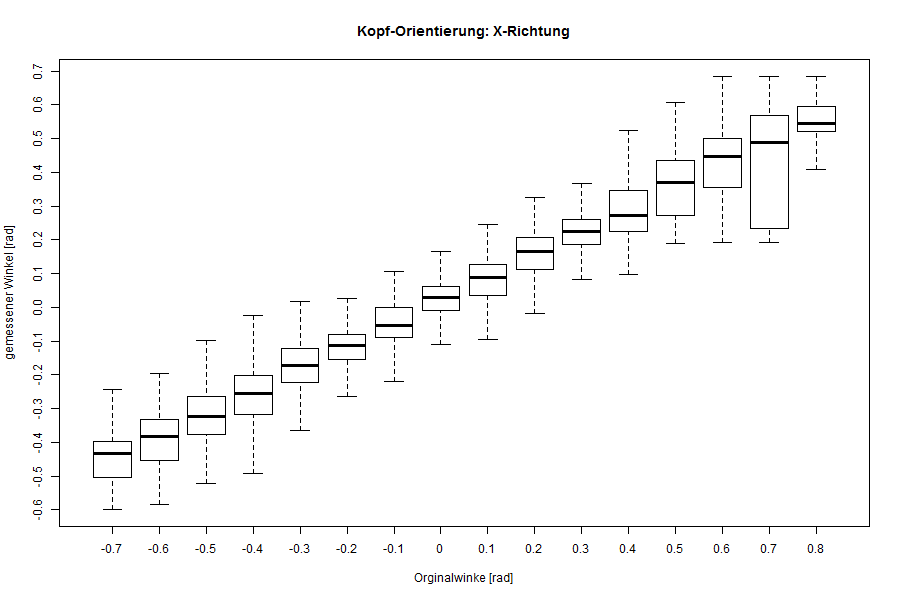
\includegraphics[width=0.192\linewidth]{OpenFace_Img/Head_x_S1}
	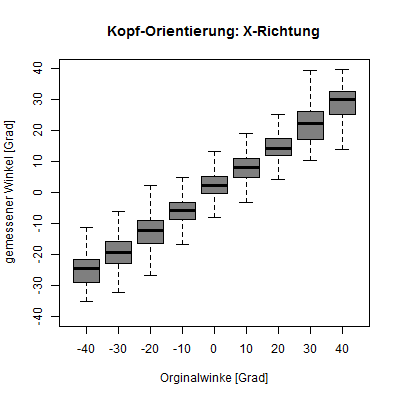
\includegraphics[width=0.192\linewidth]{OpenFace_Img/Head_x_S05}
	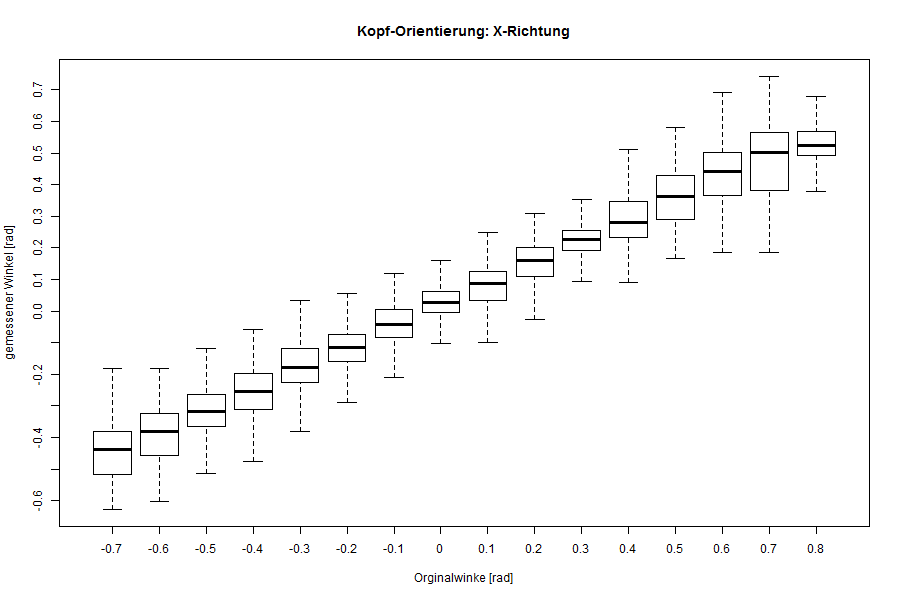
\includegraphics[width=0.192\linewidth]{OpenFace_Img/Head_x_S025}
	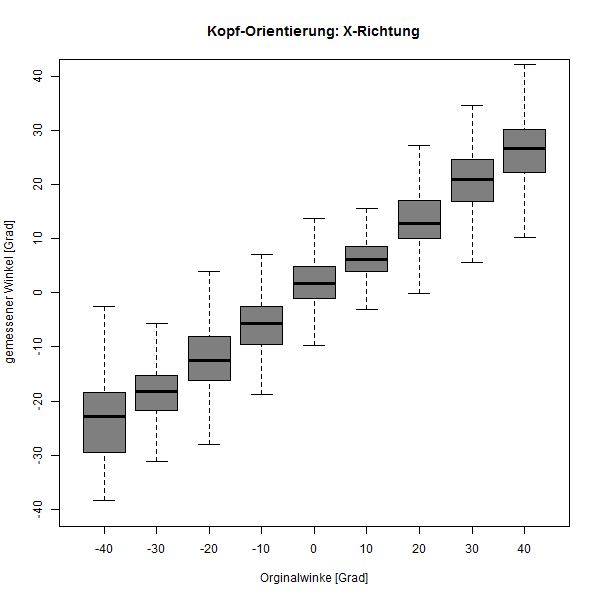
\includegraphics[width=0.192\linewidth]{OpenFace_Img/Head_x_S01}
	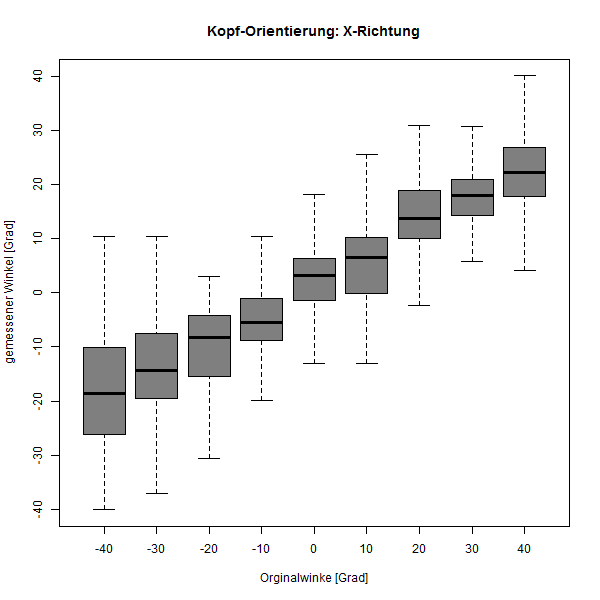
\includegraphics[width=0.192\linewidth]{OpenFace_Img/Head_x_S005}\\	
	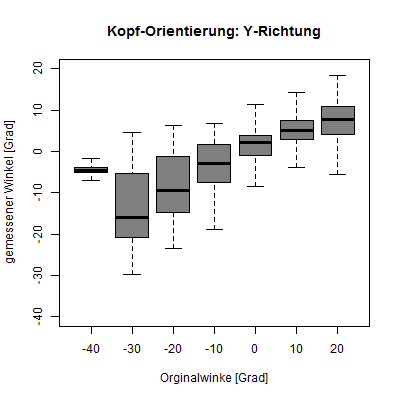
\includegraphics[width=0.192\linewidth]{OpenFace_Img/Head_y_S1}
	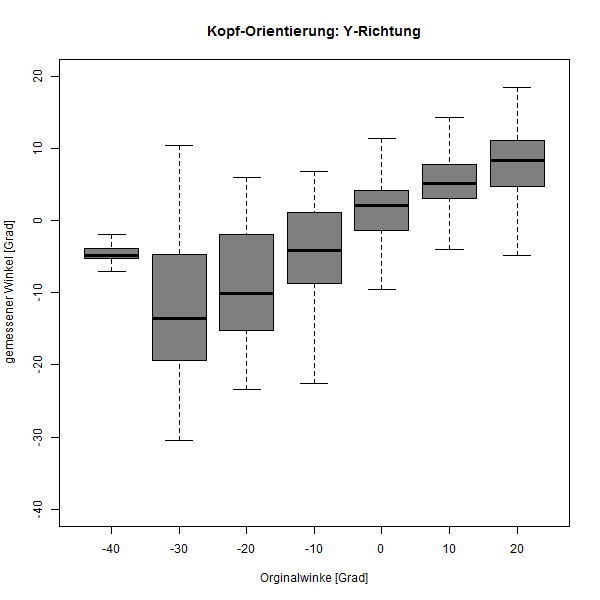
\includegraphics[width=0.192\linewidth]{OpenFace_Img/Head_y_S05}
	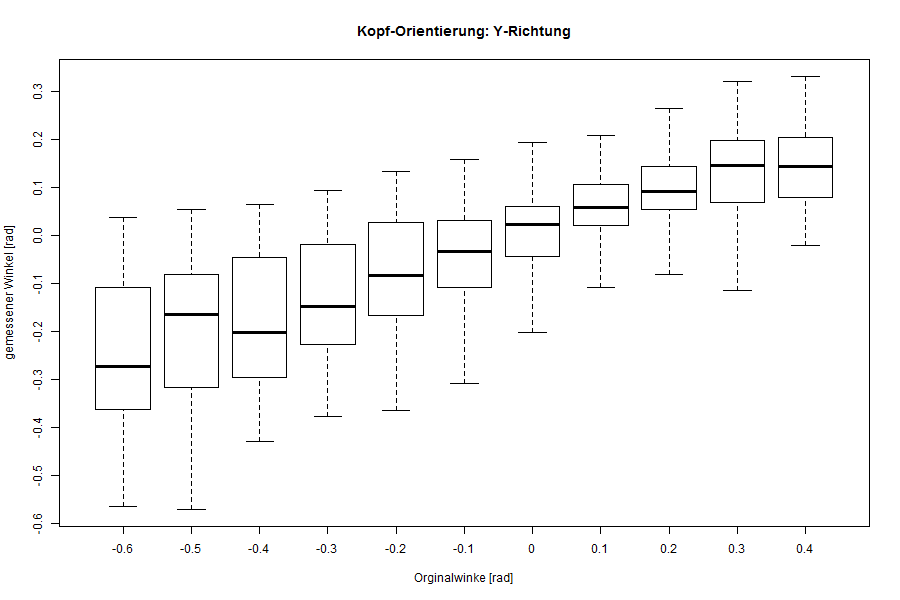
\includegraphics[width=0.192\linewidth]{OpenFace_Img/Head_y_S025}
	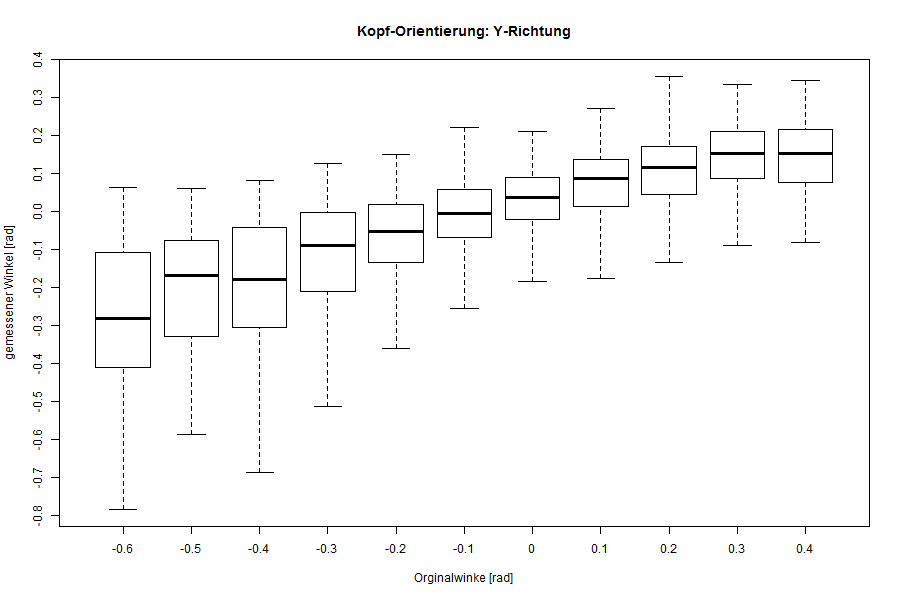
\includegraphics[width=0.192\linewidth]{OpenFace_Img/Head_y_S01}
	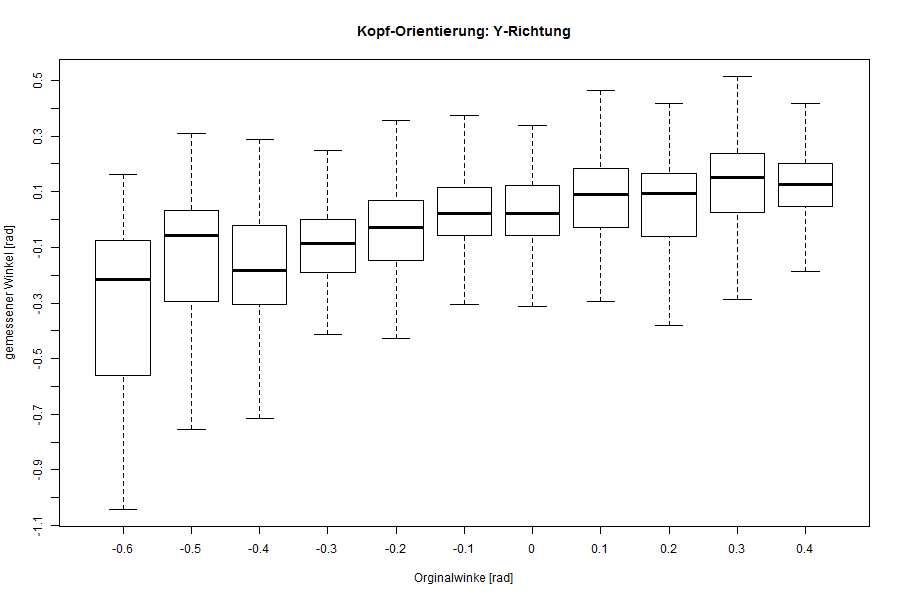
\includegraphics[width=0.192\linewidth]{OpenFace_Img/Head_y_S005}\\	
	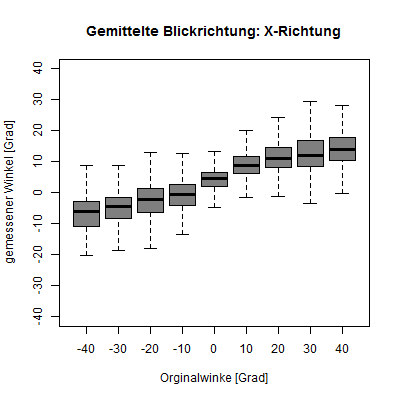
\includegraphics[width=0.192\linewidth]{OpenFace_Img/EyeAVG_x_S1}	
	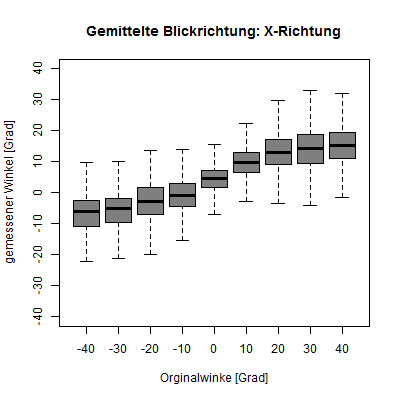
\includegraphics[width=0.192\linewidth]{OpenFace_Img/EyeAVG_x_S05}
	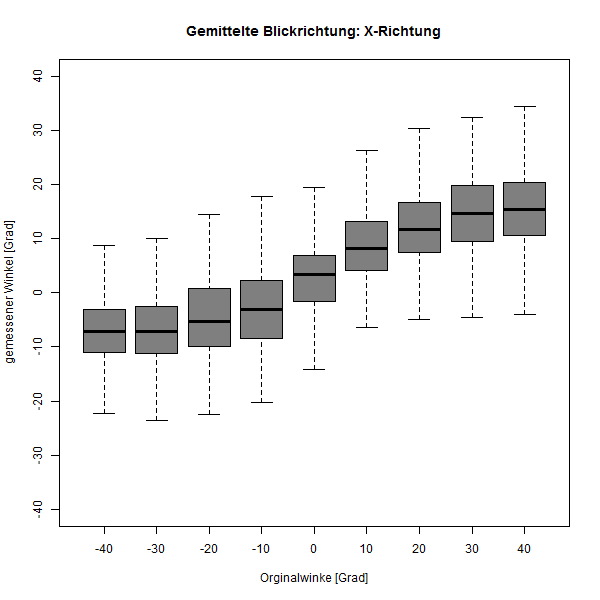
\includegraphics[width=0.192\linewidth]{OpenFace_Img/EyeAVG_x_S025}
	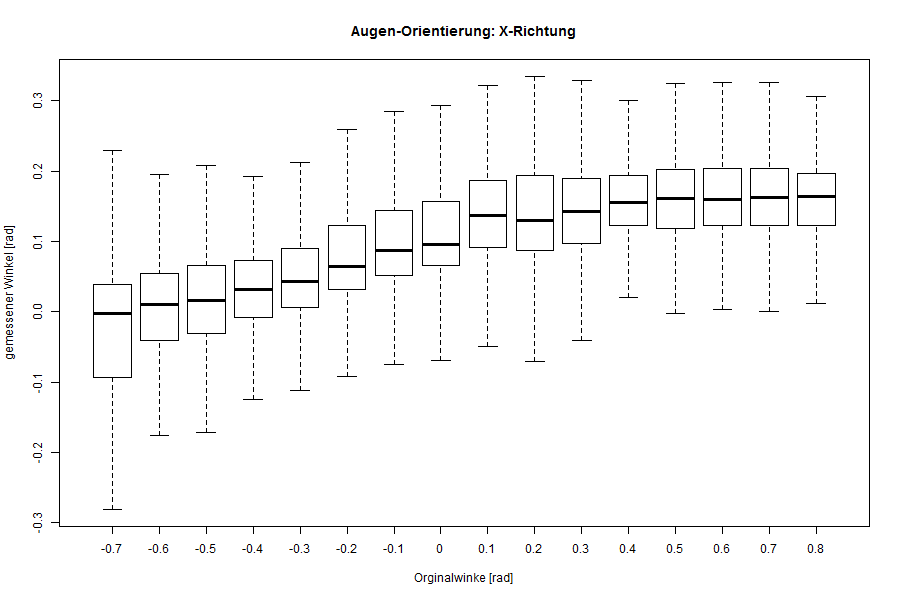
\includegraphics[width=0.192\linewidth]{OpenFace_Img/EyeAVG_x_S01}
	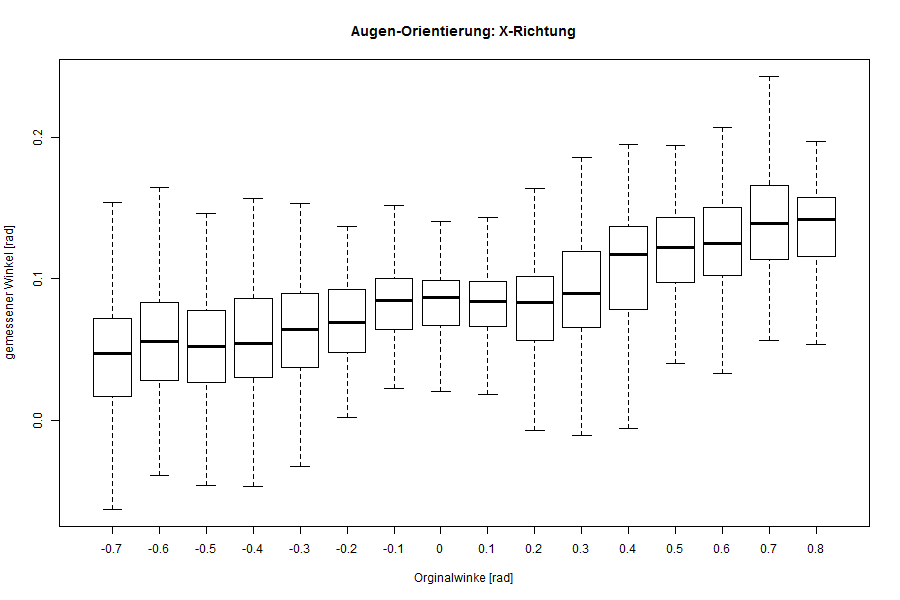
\includegraphics[width=0.192\linewidth]{OpenFace_Img/EyeAVG_x_S005}
	\caption{Auswertung der Videoaufnahme mit der Kopfausrichtung Horizontal (Oben), Kopforientierung Vertikal (Mitte) und die X-Ausrichtung der Augen (Unten)\\Skalierungsfaktor von links nach rechts (1/0.5/0.25/0.1/0.05), Y-Achse: $[0-35]^\circ$}
	\label{graph_VideoSkalierung}
\end{sidewaysfigure}
\subsection{Fehleranalyse im Versuch}
Da nur der Unterschied zwischen Target und Auftreffpunkt der gemessenen Gesichtsorientierung aufgezeigt werden kann, kommt es zu verschiedenen Fehlern. Vor allem wird der Bewegung das Targets mit den Augen gefolgt.
So wird zu Beginn der Bewegung dem Target nur mit den Augen gefolgt, bis sich der Kopf in Bewegung setzt. Dies wird so lange fortgeführt, bis die Kopfdrehung unangenehm und das Ende der Bewegung des Targets absehbar wird. So wird der letzte Teil der Bewegung wieder nur von den Augen nachverfolgt.\\
Die allgemeine Exkursionen beträgt etwa $20^\circ$, der Winkelbereich der üblichen Augenbewegungen, und kann daher recht stark von der Kopforientierung abweichen.\cite{wiki_Gesichtsfeld}\\
\subsubsection{Bei der Messung}
Die erste Ungenauigkeit liegt bei der Distanz zur Leinwand, diese wurde nur vor der eigentlichen Aufnahme bestimmt. Somit entsteht eine Abweichung, da die Kopfbewegung während der Aufnahme nicht erfasst wird.\\
Die eigentliche Messung der Distanz  vom Kopf der Personen zur Leinwand ist ebenfalls ungenau, da sie eine Abweichung von etwa $1cm$ in alle Richtungen aufweist. Außerdem liegt der Ursprung des Kopfes in der Anwendung etwas tiefer und weiter hinten als der ausgemessene Nasenrücken.\\
Auch die Parameter für die Überführungsmatrix von Welt- nach Kamerakoordinaten sowie die Brennweite wurden zwar sorgsam bestimmt, sind aber dennoch nicht perfekt.\\
Bedingt durch den Aufbau und der verwendeten Hardware, musste die Kamera in Richtung des Projektors ausgerichtet werden.  Dadurch musste diese vor dem direkten Licht geschützt des Projektors geschützt werden. Somit konnte sich die Kamera nicht im Zentrum der Messpunkte befinden.\\
Da Kamera und Leinwand fest montiert sind, ergibt sich auch die Problematik, dass der Kopf der Probanden nicht im Zentrum des Kamerabildes ist und somit hat die Kamera immer einen Blickwinkel von unten auf das Gesicht.\\
Da die Probanden ebenfalls zwischen der Leinwand und dem Projektor standen, verdeckten diese das Bild, wodurch es manchmal passierte, dass der Zielpunkt im Schatten verschwand und keine zentrale Messung mit Blickrichtung nach unten möglich ist.
\subsubsection{Umgebung}
Bei der Aufzeichnung hat sich vor allem das Problem mit der ungleichmäßigen Beleuchtung bzw. dem Gegenlicht ergeben. Diesem wurde durch Abdunkeln der Fenster und Verwendung der Tafelbeleuchtung entgegengewirkt, damit das Gesicht gut erkennbar ist. Ein Problem das auch in der realen Anwendung auftreten wird.\\
Ein weiteres allgemeines Problem ist die Anzahl der Bildpunkte des Gesichtes im Bild, somit ist eine Berechnung auf dem Gesicht zwar möglich, auf den Augen allerdings nur bedingt.\\
Außerdem wird die Auswertung der Augen weiter erschwert durch die Reflektion von starken Lichtquellen (wie z.B. Fenster, Lampen, Projektorbild) auf den Brillen, die die Pupille überdecken kann. Auch Schatten gerade in den Augenhöhlen erschweren die Auswertung.